% ---------------------------------------------------------------------------
% Material de apéndice SEPARADO del artículo.
%
% No se compila con main.tex: se conserva por si el comité o el docente pide
% los anexos. Para reincorporarlo, agregue al final de main.tex:
%
%     \appendix
%     % ---------------------------------------------------------------------------
% Material de apéndice SEPARADO del artículo.
%
% No se compila con main.tex: se conserva por si el comité o el docente pide
% los anexos. Para reincorporarlo, agregue al final de main.tex:
%
%     \appendix
%     % ---------------------------------------------------------------------------
% Material de apéndice SEPARADO del artículo.
%
% No se compila con main.tex: se conserva por si el comité o el docente pide
% los anexos. Para reincorporarlo, agregue al final de main.tex:
%
%     \appendix
%     % ---------------------------------------------------------------------------
% Material de apéndice SEPARADO del artículo.
%
% No se compila con main.tex: se conserva por si el comité o el docente pide
% los anexos. Para reincorporarlo, agregue al final de main.tex:
%
%     \appendix
%     \input{apendices_opcionales}
%
% Requiere \tk{} y la figura derivación definidas en el preámbulo.
% ---------------------------------------------------------------------------

\section{Derivación del contrapunteo}
\label{app:derivacion}

El árbol de derivación de \tk{TDSDTSDTF} corresponde a un contrapunteo con $n=2$ ciclos. La regla $\langle bordoneo\rangle\to\tk{SDT}\langle bordoneo\rangle$ se aplica una vez y luego se cierra con $\langle bordoneo\rangle\to\tk{SDT}$. El árbol hace visible que la cadena tiene una estructura de dos bloques y que el cierre con \texttt{F} es el último paso.

\begin{figure}[t]
\centering
\resizebox{\columnwidth}{!}{%
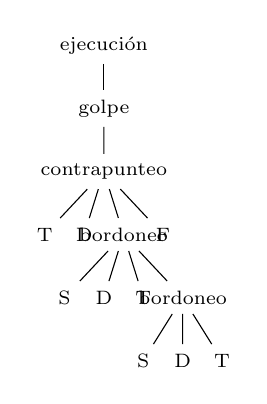
\begin{tikzpicture}[
  level distance=8mm,
  sibling distance=5mm,
  every node/.style={font=\scriptsize},
  edge from parent/.style={draw}
]
\node {ejecución}
  child {node {golpe}
    child {node {contrapunteo}
      child {node {\tk{T}}}
      child {node {\tk{D}}}
      child {node {bordoneo}
        child {node {\tk{S}}}
        child {node {\tk{D}}}
        child {node {\tk{T}}}
        child {node {bordoneo}
          child {node {\tk{S}}}
          child {node {\tk{D}}}
          child {node {\tk{T}}}
        }
      }
      child {node {\tk{F}}}
    }
  };
\end{tikzpicture}%
}
\caption{Árbol de derivación de \tk{TDSDTSDTF} con la gramática del juego.}
\label{fig:derivacion}
\end{figure}

La derivación completa, sin dibujar el árbol, es
\begin{align}
  \langle ejecucion\rangle
  &\Rightarrow \langle golpe\rangle
  \Rightarrow \langle contrapunteo\rangle \notag\\
  &\Rightarrow \tk{TD}\langle bordoneo\rangle\tk{F} \notag\\
  &\Rightarrow \tk{TDSDT}\langle bordoneo\rangle\tk{F} \notag\\
  &\Rightarrow \tk{TDSDTSDTF}.
  \label{eq:derivacion}
\end{align}
Cada paso aplica una única producción y consume exactamente un bloque \tk{SDT}; por eso la derivación es única.

\section{Tabla de transición de la máquina}
\label{app:delta}

La tabla siguiente tabula la función $\delta$ para el caso en que la acción del jugador es distinta de la anterior, de modo que $r'=1$ y $q_d$ es el estado que corresponde a cada decisión. Las columnas $f$ y $f'$ son la furia antes y después; $d$ es la decisión escrita en la tercera cinta. Si la acción se repite, $r'=\min(r+1,3)$, y la decisión es \texttt{CASTIGO} cuando $r'=3$, con prioridad sobre las demás reglas.

\begin{table}[t]
\centering
\caption{Transición de la máquina para $a\neq$ acción anterior ($r'=1$).}
\label{tab:delta}
\setlength{\tabcolsep}{4pt}
\begin{tabular}{c c c c l}
\toprule
\textbf{$a$} & \textbf{$f$} & \textbf{$f'$} & \textbf{$r'$} & \textbf{$d$} \\
\midrule
A & 0 & 1 & 1 & ATAQUE\_RAPIDO \\
A & 1 & 2 & 1 & ATAQUE\_PESADO \\
A & 2 & 3 & 1 & ATAQUE\_PESADO \\
A & 3 & 3 & 1 & ATAQUE\_PESADO \\
\midrule
D & 0 & 0 & 1 & BLOQUEO \\
D & 1 & 0 & 1 & BLOQUEO \\
D & 2 & 1 & 1 & BLOQUEO \\
D & 3 & 2 & 1 & BLOQUEO \\
\midrule
C & 0 & 0 & 1 & ATAQUE\_RAPIDO \\
C & 1 & 0 & 1 & ATAQUE\_RAPIDO \\
C & 2 & 1 & 1 & ATAQUE\_RAPIDO \\
C & 3 & 2 & 1 & ATAQUE\_RAPIDO \\
\midrule
E & 0 & 2 & 1 & CASTIGO \\
E & 1 & 3 & 1 & CASTIGO \\
E & 2 & 3 & 1 & CASTIGO \\
E & 3 & 3 & 1 & CASTIGO \\
\bottomrule
\end{tabular}
\end{table}

\section{Traza de una petición}
\label{app:traza}

La siguiente traza corresponde a \tk{TDDTF} desde una partida nueva. El cliente envía
\begin{verbatim}
{"secuencia":"TDDTF"}
\end{verbatim}
y el servidor responde con una línea JSON:
\begin{verbatim}
{"contrato_version":"1.0","valido":true,
 "golpe":"Golpe de Gaban","accion":"A","error":null,
 "dano_enemigo":15,"dano_jugador":10,
 "enemigo_accion":"ATAQUE_RAPIDO",
 "vida_jugador":90,"vida_enemigo":85,
 "estado":"JUGANDO",
 "cintas":{"cinta1":["A"],"cinta2":["1","1"],
           "cinta3":["ATAQUE_RAPIDO"]},
 "cabezales":{"L":0,"R":0,"S":0}}
\end{verbatim}
La respuesta se puede reproducir con un cliente de consola sobre el puerto TCP 8765. El campo \texttt{cinta2} contiene la furia y la repetición; \texttt{cabezales} permite que el HUD resalte la celda actual.

%
% Requiere \tk{} y la figura derivación definidas en el preámbulo.
% ---------------------------------------------------------------------------

\section{Derivación del contrapunteo}
\label{app:derivacion}

El árbol de derivación de \tk{TDSDTSDTF} corresponde a un contrapunteo con $n=2$ ciclos. La regla $\langle bordoneo\rangle\to\tk{SDT}\langle bordoneo\rangle$ se aplica una vez y luego se cierra con $\langle bordoneo\rangle\to\tk{SDT}$. El árbol hace visible que la cadena tiene una estructura de dos bloques y que el cierre con \texttt{F} es el último paso.

\begin{figure}[t]
\centering
\resizebox{\columnwidth}{!}{%
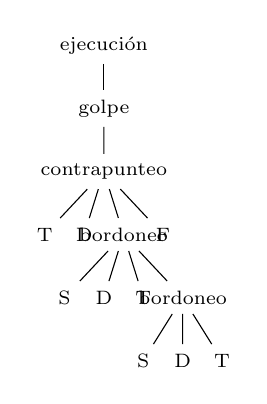
\begin{tikzpicture}[
  level distance=8mm,
  sibling distance=5mm,
  every node/.style={font=\scriptsize},
  edge from parent/.style={draw}
]
\node {ejecución}
  child {node {golpe}
    child {node {contrapunteo}
      child {node {\tk{T}}}
      child {node {\tk{D}}}
      child {node {bordoneo}
        child {node {\tk{S}}}
        child {node {\tk{D}}}
        child {node {\tk{T}}}
        child {node {bordoneo}
          child {node {\tk{S}}}
          child {node {\tk{D}}}
          child {node {\tk{T}}}
        }
      }
      child {node {\tk{F}}}
    }
  };
\end{tikzpicture}%
}
\caption{Árbol de derivación de \tk{TDSDTSDTF} con la gramática del juego.}
\label{fig:derivacion}
\end{figure}

La derivación completa, sin dibujar el árbol, es
\begin{align}
  \langle ejecucion\rangle
  &\Rightarrow \langle golpe\rangle
  \Rightarrow \langle contrapunteo\rangle \notag\\
  &\Rightarrow \tk{TD}\langle bordoneo\rangle\tk{F} \notag\\
  &\Rightarrow \tk{TDSDT}\langle bordoneo\rangle\tk{F} \notag\\
  &\Rightarrow \tk{TDSDTSDTF}.
  \label{eq:derivacion}
\end{align}
Cada paso aplica una única producción y consume exactamente un bloque \tk{SDT}; por eso la derivación es única.

\section{Tabla de transición de la máquina}
\label{app:delta}

La tabla siguiente tabula la función $\delta$ para el caso en que la acción del jugador es distinta de la anterior, de modo que $r'=1$ y $q_d$ es el estado que corresponde a cada decisión. Las columnas $f$ y $f'$ son la furia antes y después; $d$ es la decisión escrita en la tercera cinta. Si la acción se repite, $r'=\min(r+1,3)$, y la decisión es \texttt{CASTIGO} cuando $r'=3$, con prioridad sobre las demás reglas.

\begin{table}[t]
\centering
\caption{Transición de la máquina para $a\neq$ acción anterior ($r'=1$).}
\label{tab:delta}
\setlength{\tabcolsep}{4pt}
\begin{tabular}{c c c c l}
\toprule
\textbf{$a$} & \textbf{$f$} & \textbf{$f'$} & \textbf{$r'$} & \textbf{$d$} \\
\midrule
A & 0 & 1 & 1 & ATAQUE\_RAPIDO \\
A & 1 & 2 & 1 & ATAQUE\_PESADO \\
A & 2 & 3 & 1 & ATAQUE\_PESADO \\
A & 3 & 3 & 1 & ATAQUE\_PESADO \\
\midrule
D & 0 & 0 & 1 & BLOQUEO \\
D & 1 & 0 & 1 & BLOQUEO \\
D & 2 & 1 & 1 & BLOQUEO \\
D & 3 & 2 & 1 & BLOQUEO \\
\midrule
C & 0 & 0 & 1 & ATAQUE\_RAPIDO \\
C & 1 & 0 & 1 & ATAQUE\_RAPIDO \\
C & 2 & 1 & 1 & ATAQUE\_RAPIDO \\
C & 3 & 2 & 1 & ATAQUE\_RAPIDO \\
\midrule
E & 0 & 2 & 1 & CASTIGO \\
E & 1 & 3 & 1 & CASTIGO \\
E & 2 & 3 & 1 & CASTIGO \\
E & 3 & 3 & 1 & CASTIGO \\
\bottomrule
\end{tabular}
\end{table}

\section{Traza de una petición}
\label{app:traza}

La siguiente traza corresponde a \tk{TDDTF} desde una partida nueva. El cliente envía
\begin{verbatim}
{"secuencia":"TDDTF"}
\end{verbatim}
y el servidor responde con una línea JSON:
\begin{verbatim}
{"contrato_version":"1.0","valido":true,
 "golpe":"Golpe de Gaban","accion":"A","error":null,
 "dano_enemigo":15,"dano_jugador":10,
 "enemigo_accion":"ATAQUE_RAPIDO",
 "vida_jugador":90,"vida_enemigo":85,
 "estado":"JUGANDO",
 "cintas":{"cinta1":["A"],"cinta2":["1","1"],
           "cinta3":["ATAQUE_RAPIDO"]},
 "cabezales":{"L":0,"R":0,"S":0}}
\end{verbatim}
La respuesta se puede reproducir con un cliente de consola sobre el puerto TCP 8765. El campo \texttt{cinta2} contiene la furia y la repetición; \texttt{cabezales} permite que el HUD resalte la celda actual.

%
% Requiere \tk{} y la figura derivación definidas en el preámbulo.
% ---------------------------------------------------------------------------

\section{Derivación del contrapunteo}
\label{app:derivacion}

El árbol de derivación de \tk{TDSDTSDTF} corresponde a un contrapunteo con $n=2$ ciclos. La regla $\langle bordoneo\rangle\to\tk{SDT}\langle bordoneo\rangle$ se aplica una vez y luego se cierra con $\langle bordoneo\rangle\to\tk{SDT}$. El árbol hace visible que la cadena tiene una estructura de dos bloques y que el cierre con \texttt{F} es el último paso.

\begin{figure}[t]
\centering
\resizebox{\columnwidth}{!}{%
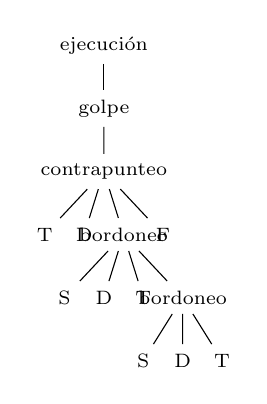
\begin{tikzpicture}[
  level distance=8mm,
  sibling distance=5mm,
  every node/.style={font=\scriptsize},
  edge from parent/.style={draw}
]
\node {ejecución}
  child {node {golpe}
    child {node {contrapunteo}
      child {node {\tk{T}}}
      child {node {\tk{D}}}
      child {node {bordoneo}
        child {node {\tk{S}}}
        child {node {\tk{D}}}
        child {node {\tk{T}}}
        child {node {bordoneo}
          child {node {\tk{S}}}
          child {node {\tk{D}}}
          child {node {\tk{T}}}
        }
      }
      child {node {\tk{F}}}
    }
  };
\end{tikzpicture}%
}
\caption{Árbol de derivación de \tk{TDSDTSDTF} con la gramática del juego.}
\label{fig:derivacion}
\end{figure}

La derivación completa, sin dibujar el árbol, es
\begin{align}
  \langle ejecucion\rangle
  &\Rightarrow \langle golpe\rangle
  \Rightarrow \langle contrapunteo\rangle \notag\\
  &\Rightarrow \tk{TD}\langle bordoneo\rangle\tk{F} \notag\\
  &\Rightarrow \tk{TDSDT}\langle bordoneo\rangle\tk{F} \notag\\
  &\Rightarrow \tk{TDSDTSDTF}.
  \label{eq:derivacion}
\end{align}
Cada paso aplica una única producción y consume exactamente un bloque \tk{SDT}; por eso la derivación es única.

\section{Tabla de transición de la máquina}
\label{app:delta}

La tabla siguiente tabula la función $\delta$ para el caso en que la acción del jugador es distinta de la anterior, de modo que $r'=1$ y $q_d$ es el estado que corresponde a cada decisión. Las columnas $f$ y $f'$ son la furia antes y después; $d$ es la decisión escrita en la tercera cinta. Si la acción se repite, $r'=\min(r+1,3)$, y la decisión es \texttt{CASTIGO} cuando $r'=3$, con prioridad sobre las demás reglas.

\begin{table}[t]
\centering
\caption{Transición de la máquina para $a\neq$ acción anterior ($r'=1$).}
\label{tab:delta}
\setlength{\tabcolsep}{4pt}
\begin{tabular}{c c c c l}
\toprule
\textbf{$a$} & \textbf{$f$} & \textbf{$f'$} & \textbf{$r'$} & \textbf{$d$} \\
\midrule
A & 0 & 1 & 1 & ATAQUE\_RAPIDO \\
A & 1 & 2 & 1 & ATAQUE\_PESADO \\
A & 2 & 3 & 1 & ATAQUE\_PESADO \\
A & 3 & 3 & 1 & ATAQUE\_PESADO \\
\midrule
D & 0 & 0 & 1 & BLOQUEO \\
D & 1 & 0 & 1 & BLOQUEO \\
D & 2 & 1 & 1 & BLOQUEO \\
D & 3 & 2 & 1 & BLOQUEO \\
\midrule
C & 0 & 0 & 1 & ATAQUE\_RAPIDO \\
C & 1 & 0 & 1 & ATAQUE\_RAPIDO \\
C & 2 & 1 & 1 & ATAQUE\_RAPIDO \\
C & 3 & 2 & 1 & ATAQUE\_RAPIDO \\
\midrule
E & 0 & 2 & 1 & CASTIGO \\
E & 1 & 3 & 1 & CASTIGO \\
E & 2 & 3 & 1 & CASTIGO \\
E & 3 & 3 & 1 & CASTIGO \\
\bottomrule
\end{tabular}
\end{table}

\section{Traza de una petición}
\label{app:traza}

La siguiente traza corresponde a \tk{TDDTF} desde una partida nueva. El cliente envía
\begin{verbatim}
{"secuencia":"TDDTF"}
\end{verbatim}
y el servidor responde con una línea JSON:
\begin{verbatim}
{"contrato_version":"1.0","valido":true,
 "golpe":"Golpe de Gaban","accion":"A","error":null,
 "dano_enemigo":15,"dano_jugador":10,
 "enemigo_accion":"ATAQUE_RAPIDO",
 "vida_jugador":90,"vida_enemigo":85,
 "estado":"JUGANDO",
 "cintas":{"cinta1":["A"],"cinta2":["1","1"],
           "cinta3":["ATAQUE_RAPIDO"]},
 "cabezales":{"L":0,"R":0,"S":0}}
\end{verbatim}
La respuesta se puede reproducir con un cliente de consola sobre el puerto TCP 8765. El campo \texttt{cinta2} contiene la furia y la repetición; \texttt{cabezales} permite que el HUD resalte la celda actual.

%
% Requiere \tk{} y la figura derivación definidas en el preámbulo.
% ---------------------------------------------------------------------------

\section{Derivación del contrapunteo}
\label{app:derivacion}

El árbol de derivación de \tk{TDSDTSDTF} corresponde a un contrapunteo con $n=2$ ciclos. La regla $\langle bordoneo\rangle\to\tk{SDT}\langle bordoneo\rangle$ se aplica una vez y luego se cierra con $\langle bordoneo\rangle\to\tk{SDT}$. El árbol hace visible que la cadena tiene una estructura de dos bloques y que el cierre con \texttt{F} es el último paso.

\begin{figure}[t]
\centering
\resizebox{\columnwidth}{!}{%
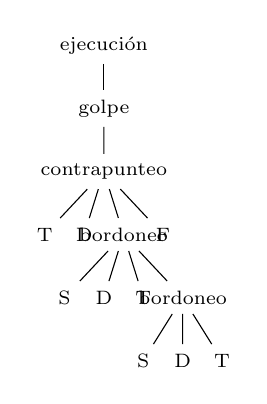
\begin{tikzpicture}[
  level distance=8mm,
  sibling distance=5mm,
  every node/.style={font=\scriptsize},
  edge from parent/.style={draw}
]
\node {ejecución}
  child {node {golpe}
    child {node {contrapunteo}
      child {node {\tk{T}}}
      child {node {\tk{D}}}
      child {node {bordoneo}
        child {node {\tk{S}}}
        child {node {\tk{D}}}
        child {node {\tk{T}}}
        child {node {bordoneo}
          child {node {\tk{S}}}
          child {node {\tk{D}}}
          child {node {\tk{T}}}
        }
      }
      child {node {\tk{F}}}
    }
  };
\end{tikzpicture}%
}
\caption{Árbol de derivación de \tk{TDSDTSDTF} con la gramática del juego.}
\label{fig:derivacion}
\end{figure}

La derivación completa, sin dibujar el árbol, es
\begin{align}
  \langle ejecucion\rangle
  &\Rightarrow \langle golpe\rangle
  \Rightarrow \langle contrapunteo\rangle \notag\\
  &\Rightarrow \tk{TD}\langle bordoneo\rangle\tk{F} \notag\\
  &\Rightarrow \tk{TDSDT}\langle bordoneo\rangle\tk{F} \notag\\
  &\Rightarrow \tk{TDSDTSDTF}.
  \label{eq:derivacion}
\end{align}
Cada paso aplica una única producción y consume exactamente un bloque \tk{SDT}; por eso la derivación es única.

\section{Tabla de transición de la máquina}
\label{app:delta}

La tabla siguiente tabula la función $\delta$ para el caso en que la acción del jugador es distinta de la anterior, de modo que $r'=1$ y $q_d$ es el estado que corresponde a cada decisión. Las columnas $f$ y $f'$ son la furia antes y después; $d$ es la decisión escrita en la tercera cinta. Si la acción se repite, $r'=\min(r+1,3)$, y la decisión es \texttt{CASTIGO} cuando $r'=3$, con prioridad sobre las demás reglas.

\begin{table}[t]
\centering
\caption{Transición de la máquina para $a\neq$ acción anterior ($r'=1$).}
\label{tab:delta}
\setlength{\tabcolsep}{4pt}
\begin{tabular}{c c c c l}
\toprule
\textbf{$a$} & \textbf{$f$} & \textbf{$f'$} & \textbf{$r'$} & \textbf{$d$} \\
\midrule
A & 0 & 1 & 1 & ATAQUE\_RAPIDO \\
A & 1 & 2 & 1 & ATAQUE\_PESADO \\
A & 2 & 3 & 1 & ATAQUE\_PESADO \\
A & 3 & 3 & 1 & ATAQUE\_PESADO \\
\midrule
D & 0 & 0 & 1 & BLOQUEO \\
D & 1 & 0 & 1 & BLOQUEO \\
D & 2 & 1 & 1 & BLOQUEO \\
D & 3 & 2 & 1 & BLOQUEO \\
\midrule
C & 0 & 0 & 1 & ATAQUE\_RAPIDO \\
C & 1 & 0 & 1 & ATAQUE\_RAPIDO \\
C & 2 & 1 & 1 & ATAQUE\_RAPIDO \\
C & 3 & 2 & 1 & ATAQUE\_RAPIDO \\
\midrule
E & 0 & 2 & 1 & CASTIGO \\
E & 1 & 3 & 1 & CASTIGO \\
E & 2 & 3 & 1 & CASTIGO \\
E & 3 & 3 & 1 & CASTIGO \\
\bottomrule
\end{tabular}
\end{table}

\section{Traza de una petición}
\label{app:traza}

La siguiente traza corresponde a \tk{TDDTF} desde una partida nueva. El cliente envía
\begin{verbatim}
{"secuencia":"TDDTF"}
\end{verbatim}
y el servidor responde con una línea JSON:
\begin{verbatim}
{"contrato_version":"1.0","valido":true,
 "golpe":"Golpe de Gaban","accion":"A","error":null,
 "dano_enemigo":15,"dano_jugador":10,
 "enemigo_accion":"ATAQUE_RAPIDO",
 "vida_jugador":90,"vida_enemigo":85,
 "estado":"JUGANDO",
 "cintas":{"cinta1":["A"],"cinta2":["1","1"],
           "cinta3":["ATAQUE_RAPIDO"]},
 "cabezales":{"L":0,"R":0,"S":0}}
\end{verbatim}
La respuesta se puede reproducir con un cliente de consola sobre el puerto TCP 8765. El campo \texttt{cinta2} contiene la furia y la repetición; \texttt{cabezales} permite que el HUD resalte la celda actual.
